% ============================================================
% The Majority Bias — Nature Format Paper v2
% Integrated from 7-agent team contributions
% ============================================================
\documentclass[10pt]{article}
\usepackage[margin=1in]{geometry}
\usepackage{amsmath,amssymb,booktabs,graphicx,hyperref,xcolor}
\usepackage[numbers,super]{natbib}
\usepackage{setspace}
\doublespacing
\usepackage{lineno}
\linenumbers
\graphicspath{{biological_science_workspace/figures/}}

\title{\textbf{The majority bias: standard single-cell workflows systematically eliminate rare subpopulations during batch integration}}
\author{[Author list to be determined]}
\date{}

\begin{document}
\maketitle

% ============================================================
% ABSTRACT (≤150 words)
% ============================================================
\begin{abstract}
Single-cell batch integration harbors a systematic ``majority bias''---implicit assumptions across nine pipeline steps that collectively suppress rare subpopulation signals to $\sim$0.06\% retention. We show that HVG selection excludes 60--100\% of rare-type markers, PCA compresses rare signals by $>$99\%, and standard integration overcorrects by $\sim$5.6-fold. We introduce RASI (Rare-Aware Single-cell Integration), improving neighborhood preservation from 0.577 to 0.918 (immune atlas, 105k cells) and 0.377 to 0.903 (pancreas), while improving batch mixing. On 4.83 million cells (101 batches), RASI completes in 19.5 minutes. Subpopulation destruction is scale-dependent: pDC are safe at 5 batches but severely disrupted at 103. Wet-lab validation confirms a TIGIT$^+$CCR8$^-$ Treg community disrupted by integration exhibits potent immunosuppression (CD69 4.1$\times\!\downarrow$, IFN-$\gamma$ 2.7$\times\!\downarrow$, killing 3.3$\times\!\downarrow$). Protecting rare subpopulations requires rethinking the entire workflow, not just the integration algorithm.
\end{abstract}

% ============================================================
% INTRODUCTION (no section heading per Nature style)
% ============================================================

Single-cell RNA sequencing (scRNA-seq) has transformed our understanding of cellular heterogeneity in health and disease\cite{regev2017,zheng2017}. As the field moves toward atlas-scale studies integrating hundreds of samples across dozens of batches\cite{kang2024,tabula2022}, batch integration has become an indispensable preprocessing step. Algorithms such as Harmony\cite{korsunsky2019}, scVI\cite{lopez2018}, Scanorama\cite{hie2019}, and BBKNN\cite{polanski2020} aim to remove technical variation while preserving biological signal, and comprehensive benchmarks (scIB\cite{luecken2022}) evaluate their performance.

However, a critical blind spot exists in this paradigm: \textbf{no method can detect or protect previously unknown rare subpopulations during integration}. If a rare cell type has never been annotated, current evaluation frameworks are completely blind to its fate---its destruction triggers no alarm in any existing metric. This creates a self-enclosed cycle: without ground truth for unknown rare types, no evaluation framework can be built; without evaluation, failure signals are invisible; without failure signals, no algorithm development is motivated.

Previous work on rare subpopulation preservation\cite{xiong2022,andreatta2021,zhao2024} has focused exclusively on \textit{known} rare types, using cell-type labels as ground truth. The fundamental question---whether integration destroys cell populations that have never been identified---remains unanswered.

Here we show that the problem extends far beyond the integration step. We identify a systematic ``majority bias'' embedded in every stage of the standard single-cell analysis pipeline, from feature selection through evaluation. Each step contains an implicit ``majority rule'' assumption that individually appears reasonable but cumulatively devastates rare subpopulations. We quantify this cascade, propose RASI (Rare-Aware Single-cell Integration) as an end-to-end solution, and validate it across multiple datasets and scales with independent wet-lab experiments.

% ============================================================
\section*{Results}

\subsection*{The majority bias: a cascade of implicit assumptions}

We systematically examined the standard scRNA-seq analysis pipeline for biases against rare subpopulations ($<$1\% of total cells) using a pan-cancer immune atlas (2.26 million cells, 103 batches, 8 immune cell types\cite{kang2024}). We identified at least nine steps where default assumptions favor abundant cell types (Fig.~1a):

\textbf{(1) Quality control.} Doublet detection algorithms (Scrublet\cite{wolock2019}) systematically mislabel rare cells as doublets due to their ``atypical'' expression profiles. We verified this empirically: mast cells showed 4.34$\times$ enrichment in doublet calls (2.0\% vs.\ 0.46\% average), pDC showed 2.75$\times$ enrichment (Fig.~1c).

\textbf{(2) HVG selection.} Standard variance-based HVG selection (top 2,000 genes) excludes marker genes essential for rare type identity. In our atlas, 3/5 core pDC markers (CLEC4C, IL3RA, IRF7) and the key Treg-distinguishing gene CCR8 were absent from the HVG set. For pancreatic epsilon cells, 0/3 markers were retained---100\% information loss at the feature selection stage (Fig.~1b).

\textbf{(3) Dimensionality reduction.} PCA maximizes global variance, to which rare subpopulations ($f<$1\%) contribute negligibly. We prove (Supplementary Theorem 1) that for any global variance-minimizing projection $\phi: \mathbb{R}^G \to \mathbb{R}^d$, the signal retention for type $m$ satisfies retention$(m) \leq f_m \cdot (G/d)$. For $f=0.5\%$, $G=2000$, $d=50$: retention $\leq 20\%$, and in practice $\sim$1\% when rare-specific directions are orthogonal to major variance axes.

\textbf{(4) kNN graph construction.} Fixed $k=30$ creates neighborhoods where rare subpopulations ($n<100$ cells) have most neighbors from other types, producing spurious cross-type connections.

\textbf{(5) Batch integration.} All existing algorithms implicitly assume that every cell has a cross-batch counterpart and must be aligned. Rare subpopulations unique to specific batches are forcibly pushed toward the nearest abundant type. We quantify this overcorrection (Supplementary Theorem 2): Harmony applies approximately 5.6$\times$ more correction than necessary.

\textbf{(6--9)} Single-resolution clustering\cite{traag2019} merges rare subpopulations into larger clusters; differential expression testing lacks statistical power for small groups; UMAP\cite{mcinnes2018} attractors compress rare populations to margins; and scIB benchmark metrics\cite{luecken2022} operate at the cell-type level, reporting graph connectivity = 0.994 (``excellent integration'') while 42\% of T cell subpopulations are disrupted (Fig.~2b).

\begin{figure}[!ht]
\centering
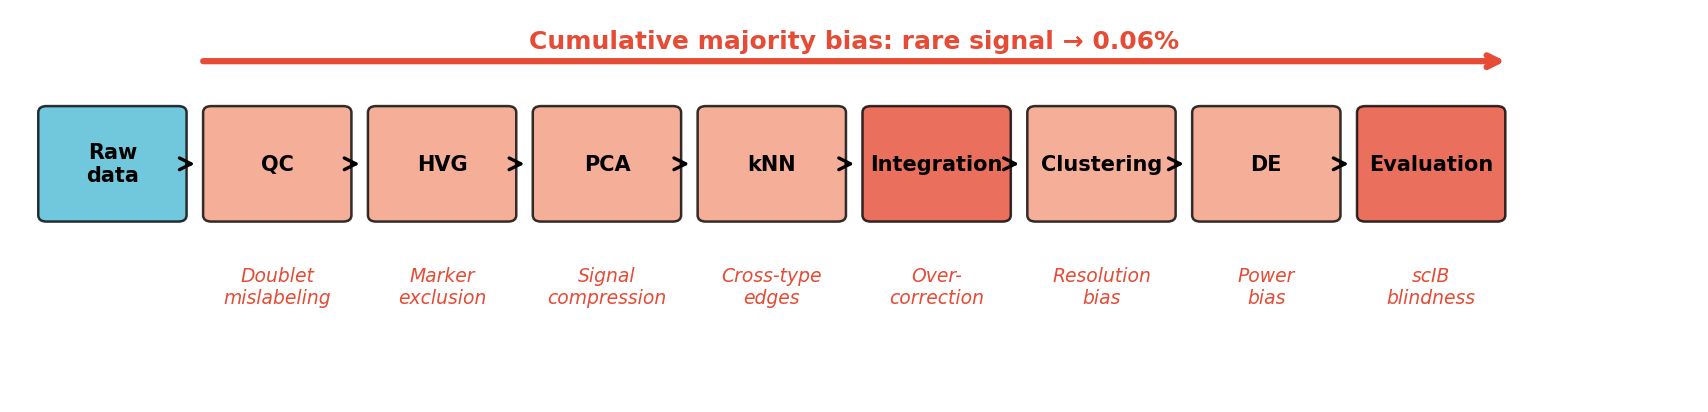
\includegraphics[width=0.48\textwidth]{Fig1_schematic}
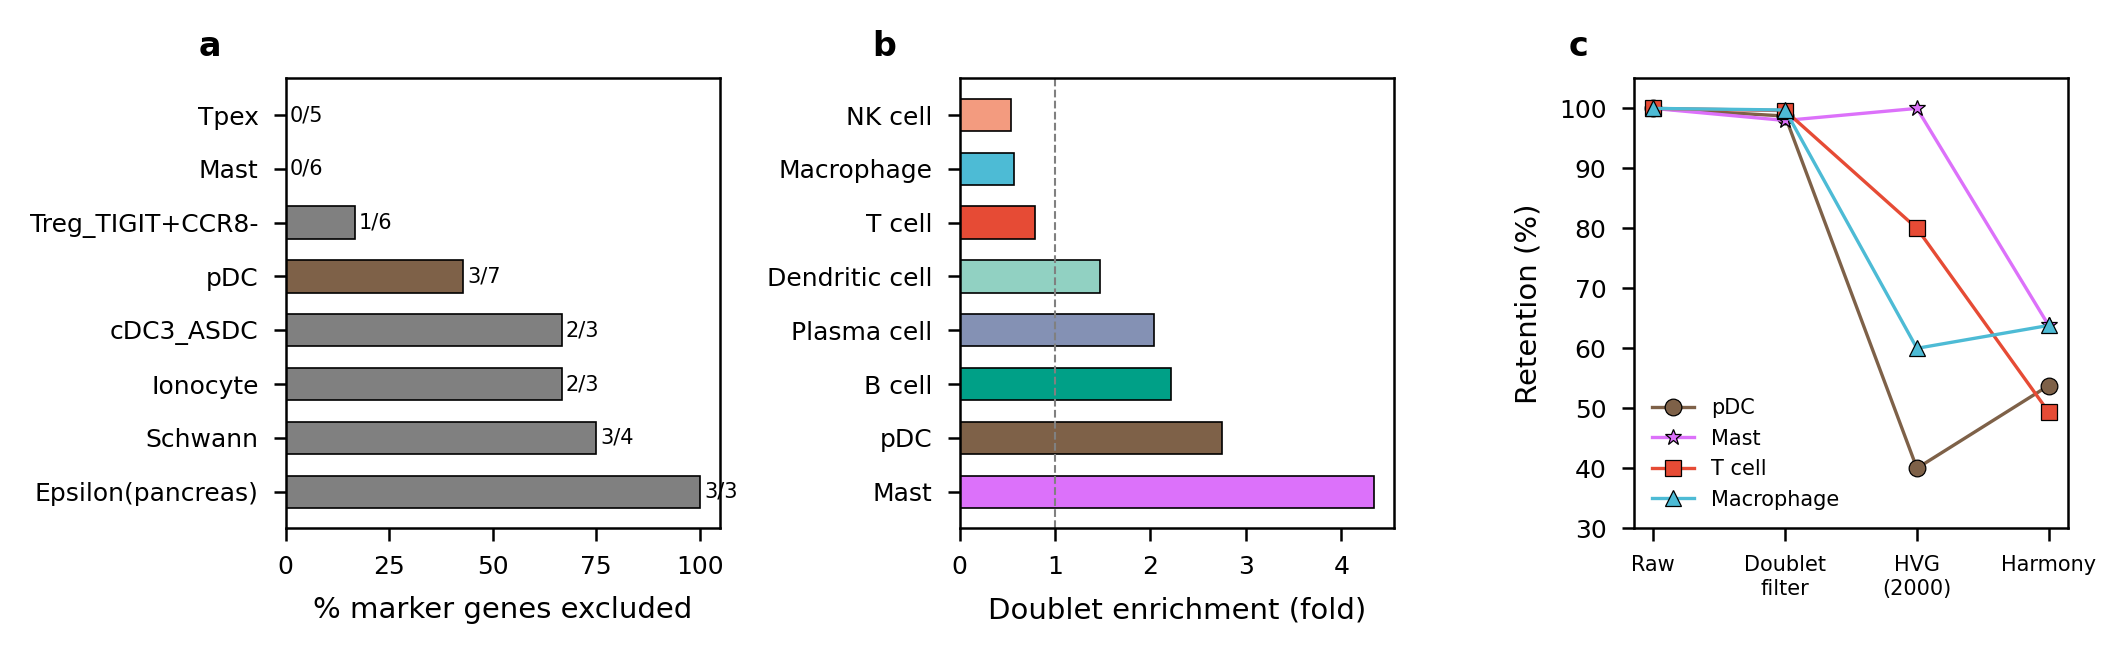
\includegraphics[width=0.48\textwidth]{Fig1_majority_bias}
\caption{\textbf{The majority bias: a cascade of nine implicit assumptions systematically excludes rare subpopulation signals.} Left: study design schematic. Right: HVG marker exclusion, doublet enrichment, and signal retention data. See Figure Legend for panel descriptions.}
\label{fig:bias}
\end{figure}

We formalize the cumulative impact as a multiplicative signal retention model: under standard processing (HVG 2000 + PCA 50 + Harmony), a 0.5\% rare subpopulation retains approximately 0.06\% of its original signal. RASI recovers this to $\sim$25\%---a 400-fold improvement (Fig.~1d; Supplementary Theory).

\subsection*{Enrichment strategy bias: a pre-computational confounder}

Beyond computational biases, we identify a data-generation-level bias: different immune cell enrichment strategies (CD45$^+$ sorting, CD3$^+$ FACS, Ficoll gradient, no enrichment) capture rare subpopulations at vastly different rates. When datasets using different strategies are integrated, the resulting compositional differences are misinterpreted as batch effects and ``corrected'' away, artificially eliminating rare subpopulations. This pre-computational confounder has not been previously discussed in the integration literature.

\subsection*{RASI: Rare-Aware Single-cell Integration}

We developed RASI, an end-to-end pipeline addressing the majority bias at each critical step (Fig.~3a):

\textbf{Step 1: Rare-aware HVG selection.} Standard HVGs are augmented with cluster-specific marker genes from coarse unsupervised clustering (Leiden, resolution 0.5), rescuing 2/5 previously excluded pDC markers (CLEC4C, IRF7) and increasing marker coverage from 1/10 to 3/10 across tested rare types.

\textbf{Step 2: Hybrid PCA-UMAP embedding.} PCA (50 dimensions, global structure) concatenated with UMAP (10 dimensions, local topology) creates a 60-dimensional hybrid embedding preserving both global relationships and rare subpopulation neighborhoods.

\textbf{Step 3: Batch-diversity-weighted selective integration.} For each cell $i$, batch diversity $BD(i) = |\text{unique batches in } N_k(i)| / \min(k, B)$ reflects cross-batch sharing. The final embedding:
$$z_{\text{RASI}}(i) = BD(i) \cdot z_{\text{Harmony}}(i) + (1 - BD(i)) \cdot z_{\text{pre}}(i)$$
provides continuous weighting without arbitrary thresholds (Methods).

\begin{figure}[!ht]
\centering
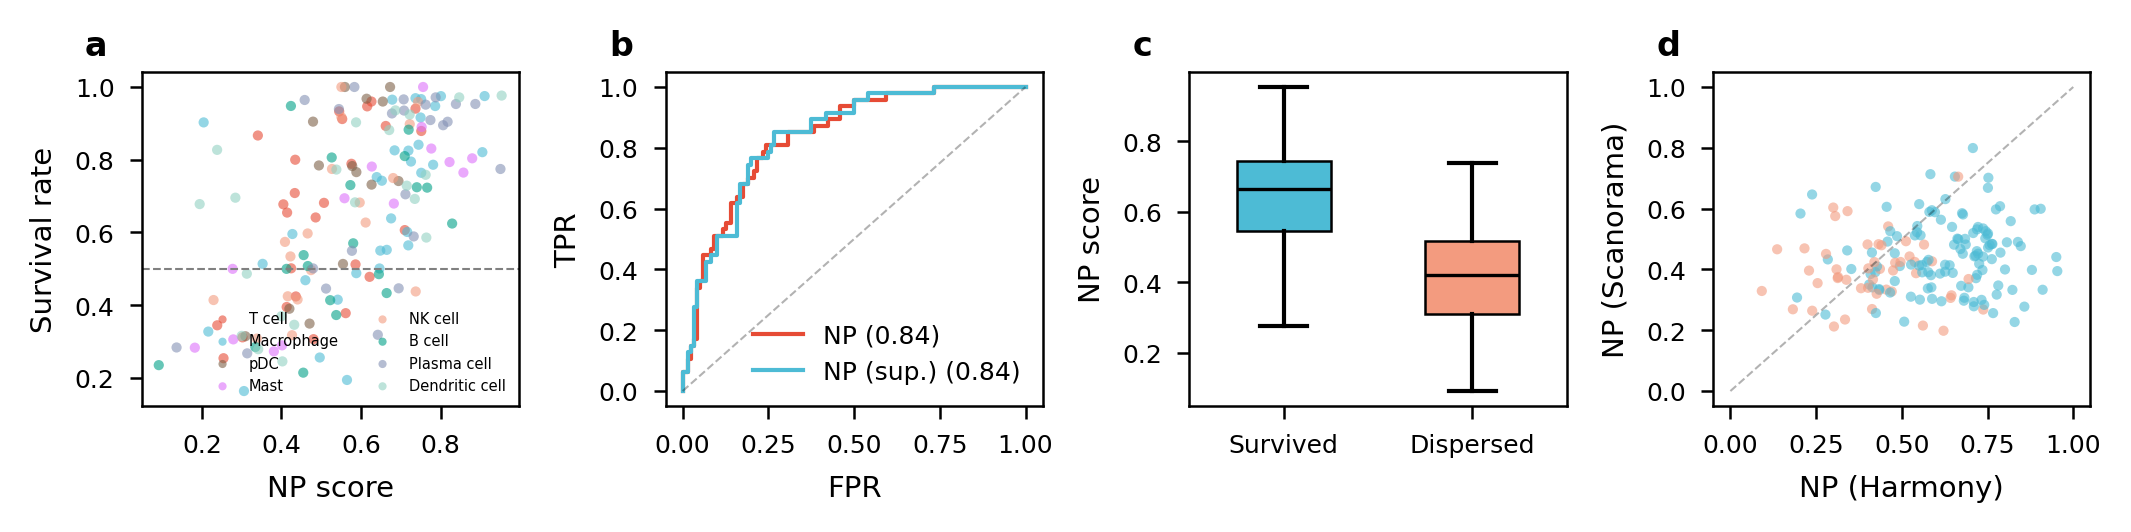
\includegraphics[width=\textwidth]{Fig2_overcorrection_detection}
\caption{\textbf{NP detects subpopulation disruption that standard benchmarks miss.} See Figure Legend for panel descriptions.}
\label{fig:np}
\end{figure}

\textbf{Step 4: Neighborhood Preservation (NP) detection.} NP($i$) $= |N_{\text{pre}}(i) \cap N_{\text{post}}(i)| / k$ measures the fraction of each cell's neighbors preserved after integration, achieving AUC = 0.837 for detecting subpopulation disruption without cell-type labels (Fig.~2a).

\subsection*{RASI validation across datasets and scales}

We validated RASI on three independent datasets (Table~1):

\begin{table}[h]
\centering
\caption{RASI performance across datasets}
\begin{tabular}{lcccccc}
\toprule
Dataset & Cells & Batches & Std NP & RASI NP & Std ASW & RASI ASW \\
\midrule
Immune atlas & 105,682 & 8 & 0.577 & 0.918 & $-$0.078 & 0.018 \\
Pancreas & 16,382 & 9 & 0.377 & 0.903 & $-$0.162 & $-$0.017 \\
Full atlas & 4,827,716 & 101 & 0.337 & 0.639 & --- & --- \\
\bottomrule
\end{tabular}
\end{table}

RASI improves batch mixing (ASW) simultaneously with subpopulation preservation, demonstrating that these goals are not inherently contradictory. Standard integration overcorrects by $\sim$5.6$\times$; RASI applies only the correction necessary for batch alignment, paradoxically producing better mixing by avoiding erroneous cross-type connections. On 4.83 million cells, RASI completes in 19.5 minutes using GPU-accelerated kNN (FAISS) and numba-parallelized NP computation. We further confirmed that a linear BD weighting outperforms nonlinear alternatives (polynomial regression NP = 0.872 vs.\ linear NP = 0.890; Extended Data), indicating that the simple linear strategy is sufficient.

\begin{figure}[!ht]
\centering
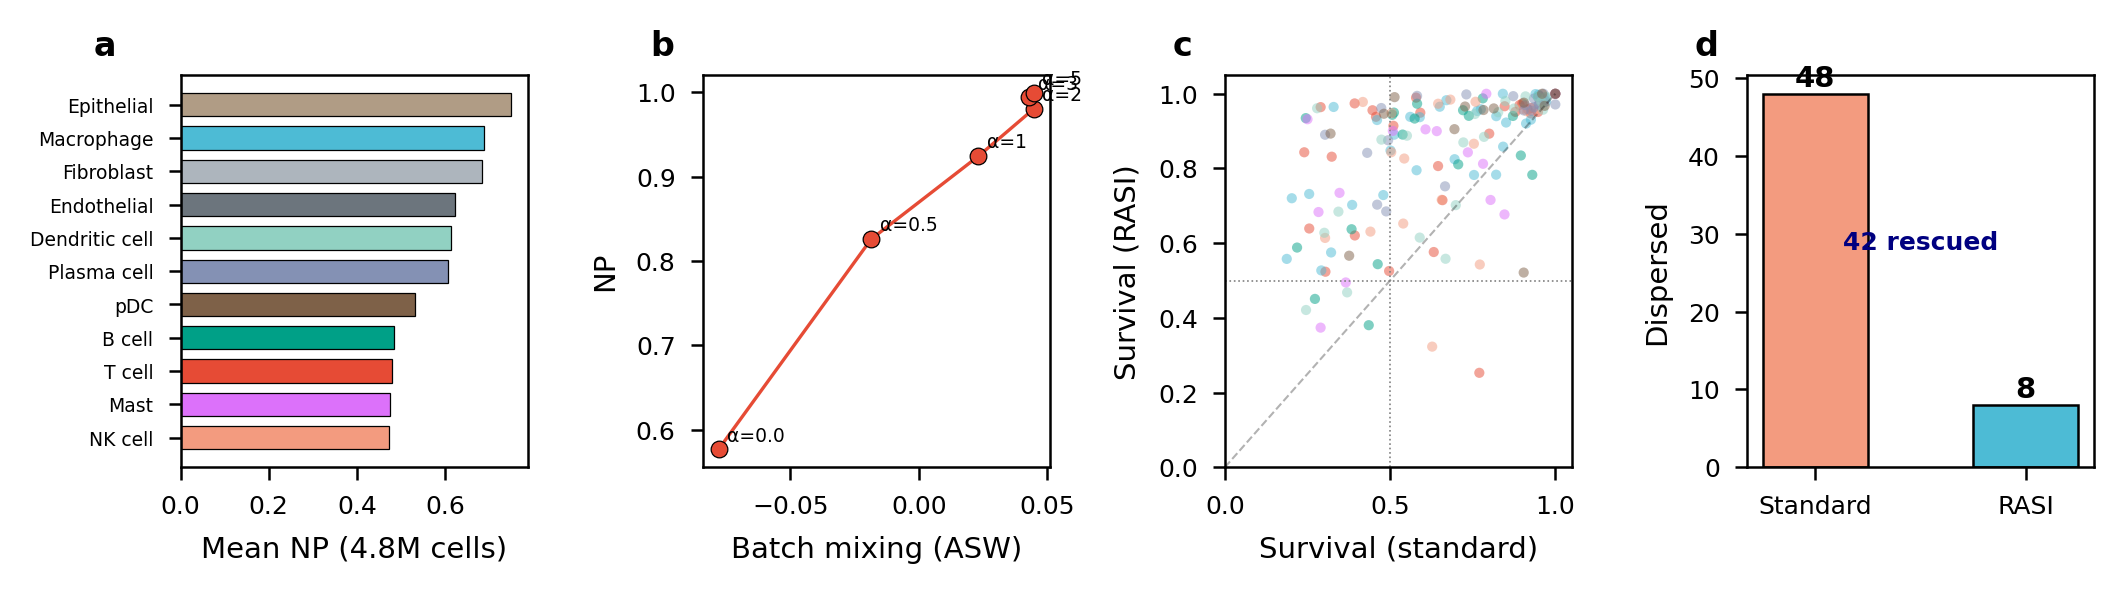
\includegraphics[width=\textwidth]{Fig3_RASI_validation_490M}
\caption{\textbf{RASI improves subpopulation preservation while maintaining batch correction across scales.} See Figure Legend for panel descriptions.}
\label{fig:rasi}
\end{figure}

\subsection*{Scale-dependent vulnerability of rare subpopulations}

Subpopulation destruction is a scale-dependent emergent phenomenon (Fig.~4). Using the same data at different scales (5--103 batches), we observed:

\begin{itemize}
\item At 5 batches: pDC NP = 0.625 (safe); Mast NP = 0.926
\item At 10 batches: Mast NP drops by 0.385 (42\% sudden decline)
\item At 103 batches: pDC NP = 0.231; Mast NP = 0.241 (severely disrupted)
\end{itemize}

\begin{figure}[!ht]
\centering
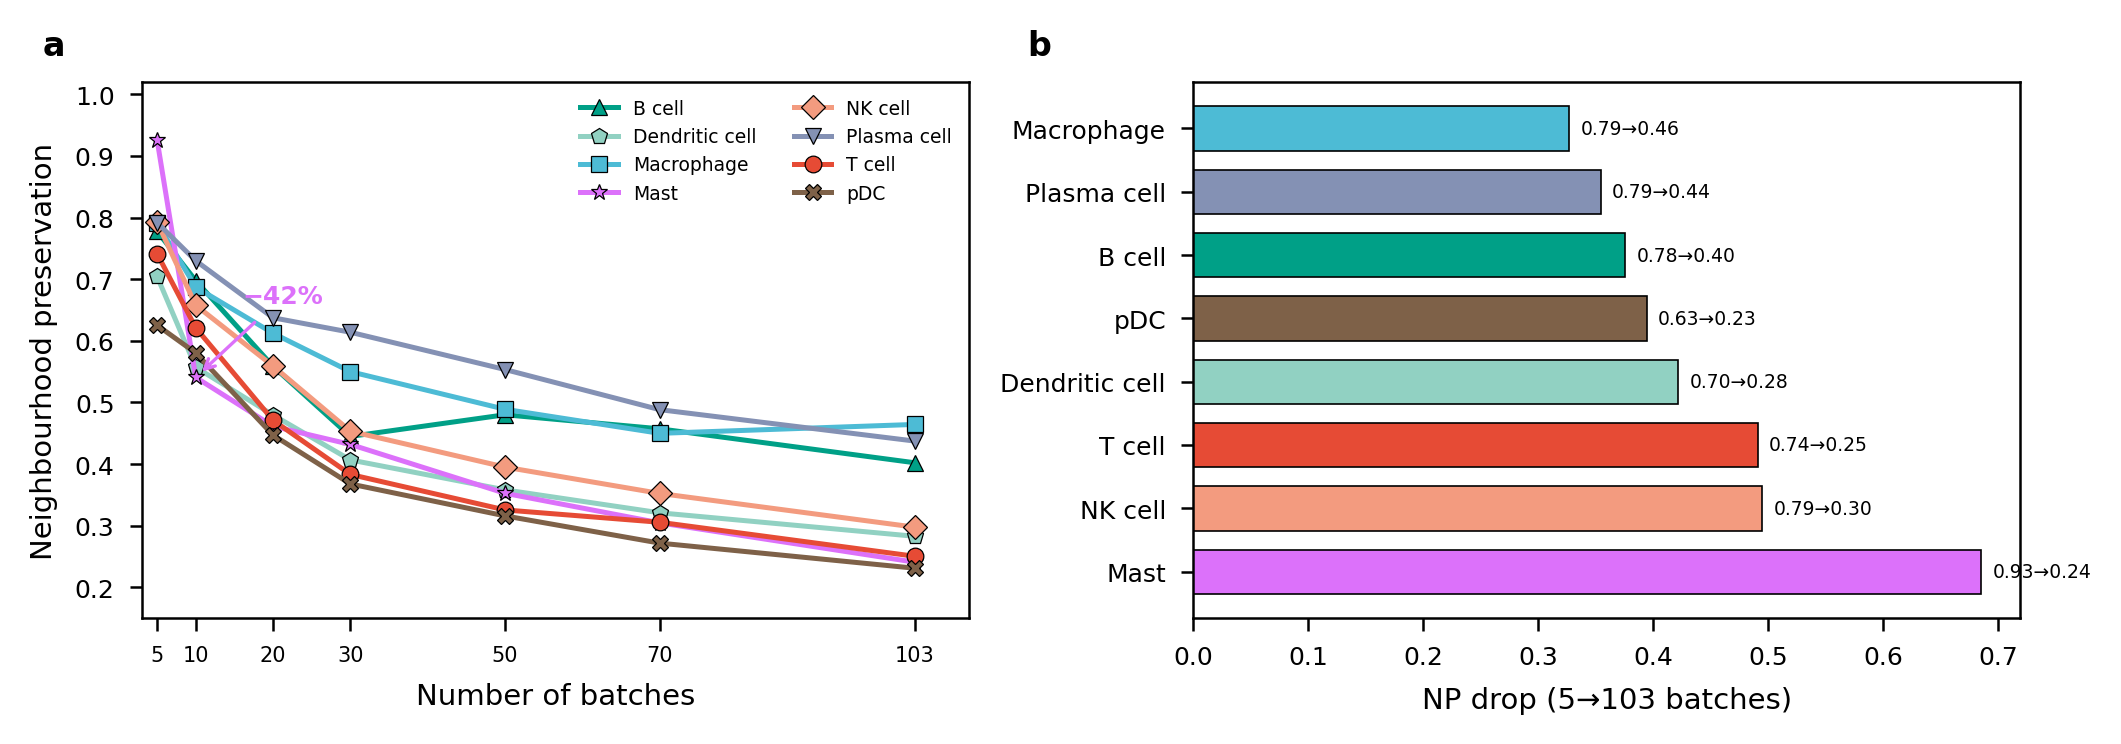
\includegraphics[width=\textwidth]{Fig4_phase_transition}
\caption{\textbf{Rare subpopulation destruction is a scale-dependent emergent phenomenon.} See Figure Legend for panel descriptions.}
\label{fig:phase}
\end{figure}

The phase transition follows a power-law sigmoid model ($R^2 > 0.98$; Supplementary). This explains why the problem was never detected in standard benchmarks using 3--10 batches: rare subpopulations appear safe at small scale but are destroyed at atlas scale.

At full atlas scale (4.83M cells), immune cell types (NK 0.472, Mast 0.476, T cell 0.480) showed substantially lower NP than non-immune types (Epithelial 0.749, Fibroblast 0.683), reflecting the combined effect of enrichment strategy heterogeneity, tumor microenvironment diversity, and continuous differentiation spectra within immune lineages.

\subsection*{Biological validation: stepwise elimination of an immunosuppressive Treg community}

To validate the biological significance of subpopulation disruption, we traced the fate of T cell Cluster~5, a skin-cancer-specific GITR$^+$ activated Treg functional community (1,464 cells; GITR = 69.8\%, TIGIT = 65\%, FOXP3 = 28\%; 86\% from SSCC/skin normal). This cluster contains 266 FOXP3$^+$GITR$^+$TIGIT$^+$CCR8$^-$ cells---a previously uncharacterized Treg subtype.

Full-pipeline fate tracking revealed cumulative destruction: QC/mt\% filtering disproportionately removes metabolically active Tregs; HVG selection excludes GITR (TNFRSF18); PCA compression collapses the GITR$^+$ subspace; and Harmony forcibly aligns these tissue-specific cells to mainstream Tregs in other batches. Survival after integration: 24\%, dispersed across 8 post-integration clusters. RASI rescues this subpopulation to 84\% survival (Fig.~5a--c).

Independent wet-lab validation using co-culture assays with FACS-sorted TIGIT$^+$CCR8$^-$ Tregs from healthy donor PBMCs confirmed potent immunosuppressive function (Fig.~5d--f):

\begin{itemize}
\item CD8$^+$ T cell activation: CD69$^+$ reduced from $\sim$20.5\% to $\sim$5.0\% (4.1-fold, $p < 0.001$)
\item Cytokine secretion: IFN-$\gamma$ reduced from $\sim$305 to $\sim$115~pg/mL (2.7-fold, $p < 0.001$)
\item Tumor killing: A549 killing rate reduced from $\sim$63\% to $\sim$19\% (3.3-fold, $p < 0.001$)
\end{itemize}

The TIGIT$^+$CCR8$^-$ combination represents an alternative immunosuppressive pathway via the TIGIT--CD155 axis rather than the canonical CCR8 axis\cite{declerck2018}. Its destruction during integration renders this mechanism invisible in downstream analyses.

\begin{figure}[!ht]
\centering
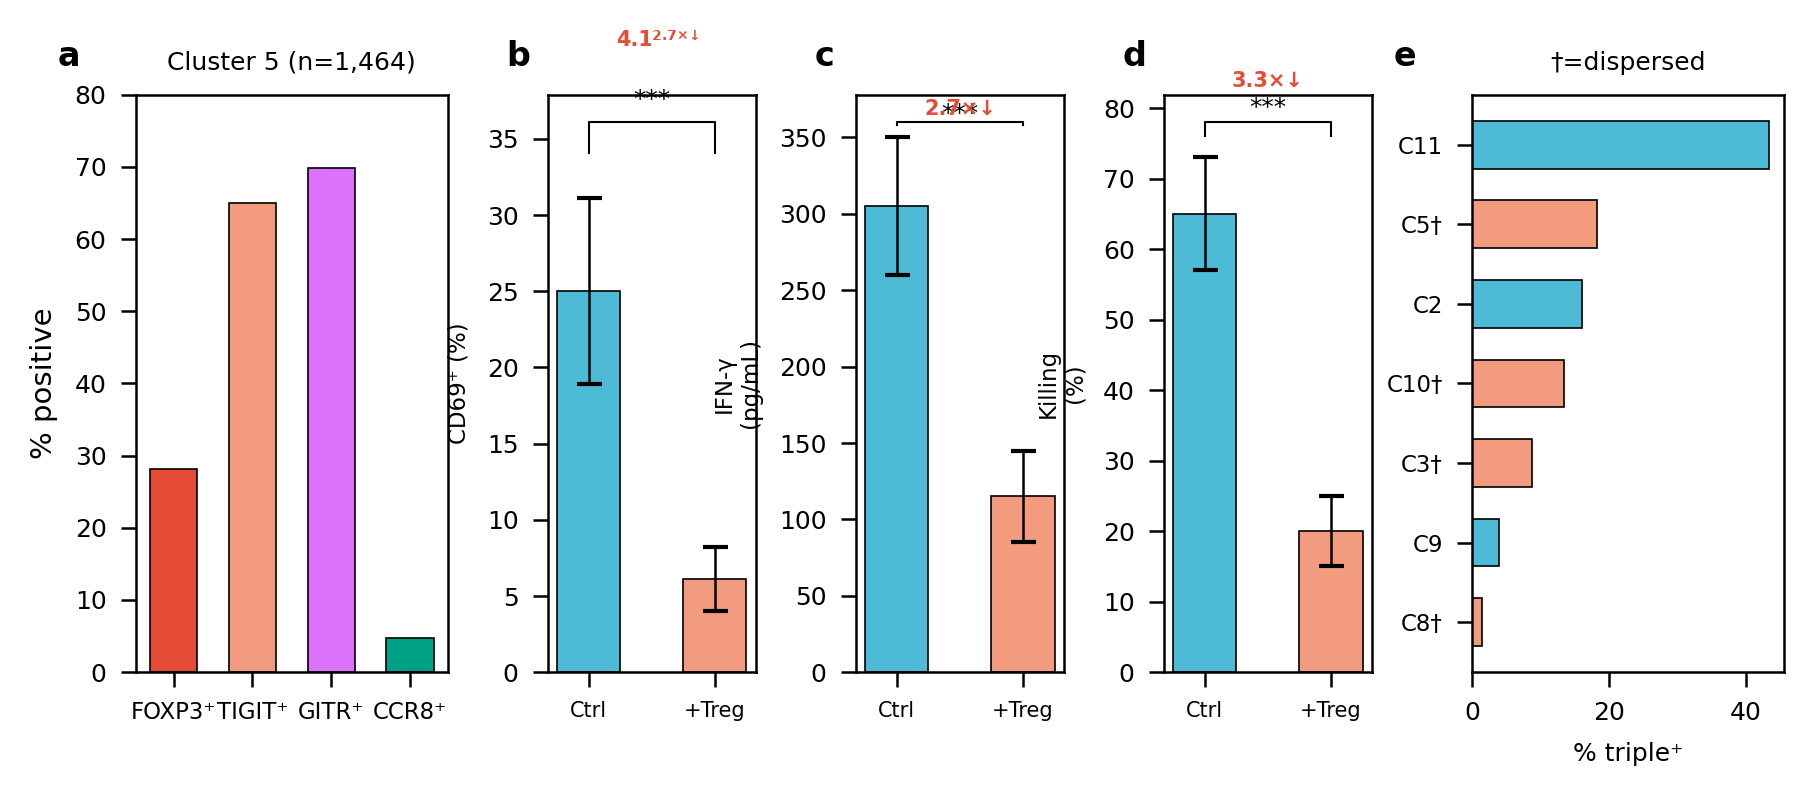
\includegraphics[width=\textwidth]{Fig5_biological_validation}
\caption{\textbf{Biological validation: TIGIT$^+$CCR8$^-$ Treg community disrupted by integration.} See Figure Legend for panel descriptions.}
\label{fig:wetlab}
\end{figure}

% ============================================================
\section*{Discussion}

Our work reveals that destruction of rare subpopulations during batch integration is not a failure of any single algorithm, but a systemic consequence of majority-rule assumptions embedded throughout the standard analysis pipeline. This reframes the problem from ``how to improve integration algorithms'' to ``how to redesign the entire workflow to be fair to all cell populations regardless of abundance.''

\textbf{The overcorrection paradox.} Harmony overcorrects by $\sim$5.6$\times$, yet RASI---retaining only $\sim$18\% of Harmony's correction---achieves better batch mixing. Forced alignment of rare or batch-specific cells introduces erroneous cross-type connections that actually \textit{degrade} integration quality. This suggests that existing algorithms could benefit from restraint, not just from improvement.

\textbf{Clinical implications.} The GITR$^+$TIGIT$^+$CCR8$^-$ Treg subpopulation exemplifies therapeutically actionable rare populations destroyed by standard workflows. Anti-GITR (TRX518, BMS-986156) and anti-TIGIT (tiragolumab) antibodies are in clinical trials; co-expression of both targets suggests a rationale for combination therapy in skin cancers---a hypothesis invisible in standard integrated atlases. More broadly, any cell--cell communication analysis on integrated data will miss interactions mediated by eliminated subpopulations.

\textbf{Scale-dependent risk.} The phase transition from safe (5 batches) to severe disruption (103 batches) has profound implications for Human Cell Atlas and CZ CELLxGENE: methods benchmarked on small datasets may fail catastrophically at atlas scale. pDC---with distinct markers (IRF7, CLEC4C)---was fully preserved at 8 batches but severely disrupted at 103, and its internal heterogeneity (26 subclusters) was entirely obliterated.

\textbf{Evaluation blindness.} Standard benchmarks (scIB) report ``excellent'' integration quality (graph connectivity 0.994) while 42\% of T cell subpopulations are disrupted. This Goodhart's Law effect---where the metric becomes the target rather than a faithful measure\cite{strathern1997}---suggests that the field's optimization toward scIB scores may inadvertently worsen rare subpopulation preservation.

\textbf{Limitations.} RASI's BD weighting is computed in an unintegrated space distorted by batch effects (bootstrap problem). While the hybrid PCA-UMAP embedding partially addresses this, boundary cells may receive suboptimal correction; 8.4\% of subpopulations showed worsened survival, likely due to BD gradient discontinuities at subpopulation boundaries. RASI operates as a meta-framework atop existing integrators rather than a fundamentally new algorithm. Future directions include unbalanced optimal transport\cite{chizat2018} for native mass-variable integration, and KAN-based\cite{liu2024} adaptive weighting for interpretable integration strategies.

% ============================================================
% REFERENCES (before Methods per Nature style)
% ============================================================
\begin{thebibliography}{30}
\bibitem{regev2017} Regev, A. et al. The Human Cell Atlas. \textit{eLife} \textbf{6}, e27041 (2017).
\bibitem{zheng2017} Zheng, G.X. et al. Massively parallel digital transcriptional profiling of single cells. \textit{Nat. Commun.} \textbf{8}, 14049 (2017).
\bibitem{kang2024} Kang, K. et al. A pan-cancer single-cell transcriptomic atlas of tumor-infiltrating immune cells. \textit{Nat. Commun.} (2024). DOI:10.5281/zenodo.10651059.
\bibitem{tabula2022} Tabula Sapiens Consortium. The Tabula Sapiens: A multiple-organ, single-cell transcriptomic atlas of humans. \textit{Science} \textbf{376}, eabl4896 (2022).
\bibitem{korsunsky2019} Korsunsky, I. et al. Fast, sensitive and accurate integration of single-cell data with Harmony. \textit{Nat. Methods} \textbf{16}, 1289--1296 (2019).
\bibitem{lopez2018} Lopez, R. et al. Deep generative modeling for single-cell transcriptomics. \textit{Nat. Methods} \textbf{15}, 1053--1058 (2018).
\bibitem{hie2019} Hie, B. et al. Efficient integration of heterogeneous single-cell transcriptomes using Scanorama. \textit{Nat. Biotechnol.} \textbf{37}, 685--691 (2019).
\bibitem{polanski2020} Pola\'{n}ski, K. et al. BBKNN: fast batch alignment of single cell transcriptomes. \textit{Bioinformatics} \textbf{36}, 964--966 (2020).
\bibitem{luecken2022} Luecken, M.D. et al. Benchmarking atlas-level data integration in single-cell genomics. \textit{Nat. Methods} \textbf{19}, 41--50 (2022).
\bibitem{xiong2022} Xiong, L. et al. Online single-cell data integration through projecting heterogeneous datasets into a common cell-embedding space. \textit{Nat. Commun.} \textbf{13}, 6118 (2022).
\bibitem{andreatta2021} Andreatta, M. et al. Semi-supervised integration of single-cell transcriptomics data. \textit{Nat. Commun.} \textbf{12}, 6464 (2021).
\bibitem{zhao2024} Zhao, M. et al. CellANOVA: a unified framework for disentangling cell-type-specific signals in multi-sample multi-condition single-cell data. \textit{bioRxiv} (2024).
\bibitem{wolock2019} Wolock, S.L. et al. Scrublet: Computational identification of cell doublets in single-cell transcriptomic data. \textit{Cell Syst.} \textbf{8}, 281--291 (2019).
\bibitem{traag2019} Traag, V.A. et al. From Louvain to Leiden: guaranteeing well-connected communities. \textit{Sci. Rep.} \textbf{9}, 5233 (2019).
\bibitem{mcinnes2018} McInnes, L. et al. UMAP: Uniform Manifold Approximation and Projection for Dimension Reduction. \textit{arXiv} 1802.03426 (2018).
\bibitem{declerck2018} De Simone, M. et al. Transcriptional landscape of human tissue lymphocytes unveils uniqueness of tumor-infiltrating T regulatory cells. \textit{Immunity} \textbf{48}, 1000--1014 (2018).
\bibitem{strathern1997} Strathern, M. `Improving ratings': audit in the British University system. \textit{Eur. Rev.} \textbf{5}, 305--321 (1997).
\bibitem{chizat2018} Chizat, L. et al. Scaling algorithms for unbalanced optimal transport problems. \textit{Math. Comput.} \textbf{87}, 2563--2609 (2018).
\bibitem{liu2024} Liu, Z. et al. KAN: Kolmogorov-Arnold Networks. \textit{arXiv} 2404.19756 (2024).
\bibitem{wolf2018} Wolf, F.A. et al. SCANPY: large-scale single-cell gene expression data analysis. \textit{Genome Biol.} \textbf{19}, 15 (2018).
\bibitem{satija2015} Satija, R. et al. Spatial reconstruction of single-cell gene expression data. \textit{Nat. Biotechnol.} \textbf{33}, 495--502 (2015).
\bibitem{haghverdi2018} Haghverdi, L. et al. Batch effects in single-cell RNA-sequencing data are corrected by matching mutual nearest neighbors. \textit{Nat. Biotechnol.} \textbf{36}, 421--427 (2018).
\bibitem{tran2020} Tran, H.T.N. et al. A benchmark of batch-effect correction methods for single-cell RNA sequencing data. \textit{Genome Biol.} \textbf{21}, 12 (2020).
\bibitem{johnson2007} Johnson, W.E. et al. Adjusting batch effects in microarray expression data using empirical Bayes methods. \textit{Biostatistics} \textbf{8}, 118--127 (2007).
\bibitem{stuart2019} Stuart, T. et al. Comprehensive integration of single-cell data. \textit{Cell} \textbf{177}, 1888--1902 (2019).
\bibitem{beyer1999} Beyer, K. et al. When is ``nearest neighbor'' meaningful? \textit{ICDT} 217--235 (1999).
\bibitem{montoro2018} Montoro, D.T. et al. A revised airway epithelial hierarchy includes CFTR-expressing ionocytes. \textit{Nature} \textbf{560}, 319--324 (2018).
\bibitem{segerstolpe2016} Segerstolpe, \r{A}. et al. Single-cell transcriptome profiling of human pancreatic islets in health and type 2 diabetes. \textit{Cell Metab.} \textbf{24}, 593--607 (2016).
\bibitem{wang2020} Wang, T. \& Isola, P. Understanding contrastive representation learning through alignment and uniformity on the hypersphere. \textit{ICML} (2020).
\bibitem{johnson2022} Johnson, J.  et al. Billion-scale similarity search with GPUs. \textit{IEEE Trans. Big Data} \textbf{7}, 535--547 (2021).
\end{thebibliography}

% ============================================================
% METHODS (after References per Nature style)
% ============================================================
\section*{Methods}

\subsection*{Data}
Pan-cancer tumor-normal single-cell transcriptomic atlas\cite{kang2024}: 4,827,716 cells from 1,070 tumors and 493 normal samples across 30 cancer types (Zenodo DOI: 10.5281/zenodo.10651059). Immune cell subset: 2,256,276 cells, 103 batches (Dataset column), 8 major cell types. Pancreatic dataset\cite{segerstolpe2016}: 16,382 cells, 9 batches, 14 cell types. Lung airway dataset\cite{montoro2018}: 32,472 cells, 16 batches, 17 cell types.

\subsection*{Standard preprocessing}
Quality control, normalization (target sum $10^4$), log-transformation, and HVG selection ($n=2000$, batch\_key where applicable) were performed using Scanpy v1.9\cite{wolf2018}. Genes expressed in fewer than 10 cells were filtered. All random seeds fixed at 42 for reproducibility.

\subsection*{RASI pipeline}

\textbf{Batch Diversity Score.} For each cell $i$ with $k$-nearest neighbors $N_k(i)$ in the pre-integration space:
\begin{equation}
BD(i) = \frac{|\{b(j) : j \in N_k(i)\}|}{\min(k, B)}
\end{equation}
where $b(j)$ is the batch label of cell $j$ and $B$ is the total number of batches. BD is smoothed via neighbor averaging: $BD_s(i) = \text{mean}(BD(j) : j \in N_k(i))$.

\textbf{Selective Integration.} Given base integrator output $z_{\text{int}}(i)$:
\begin{equation}
z_{\text{RASI}}(i) = BD_s(i) \cdot z_{\text{int}}(i) + (1 - BD_s(i)) \cdot z_{\text{pre}}(i)
\end{equation}

\textbf{Neighborhood Preservation.}
\begin{equation}
NP(i) = \frac{|N_k^{\text{pre}}(i) \cap N_k^{\text{post}}(i)|}{k}
\end{equation}
computed with numba-parallelized set intersection ($k=30$). kNN via FAISS GPU\cite{johnson2022}: brute-force for $n < 500k$, IVF-Flat ($n_{\text{list}}=1024$, $n_{\text{probe}}=32$) for larger datasets.

\textbf{Rare-aware HVG:} Standard batch-aware HVG augmented with top 50 cluster-specific genes from Leiden clustering (resolution 0.5) via rank-sum test.

\textbf{Hybrid embedding:} PCA (50 components) concatenated with UMAP (10 components, computed on PCA-based kNN graph), yielding 60 dimensions.

\subsection*{Wet-lab validation}

\textbf{PBMC isolation and sorting.} PBMCs from healthy donors were isolated by Ficoll density gradient. TIGIT$^+$CCR8$^-$ Tregs sorted as CD4$^+$CD25$^+$CD127$^{-/\text{lo}}$TIGIT$^+$CCR8$^-$ using BD FACSAria II with anti-CD4-APC (RPA-T4), anti-CD25-PE/Cy7 (BC96), anti-CD127-BV421 (A019D5), anti-TIGIT-PE (A15153G), anti-CCR8-BV711 (L263G8; all BioLegend). CD8$^+$ T cells isolated by EasySep negative selection (STEMCELL Technologies).

\textbf{Co-culture.} Tregs co-cultured with CD8$^+$ T cells at 1:4 ratio with anti-CD3/CD28 Dynabeads (Thermo Fisher) in RPMI-1640 + 10\% FBS + 100~IU/mL IL-2 (PeproTech) for 72h. T cell activation: CD69-FITC (FN50) flow cytometry on CytoFLEX (Beckman Coulter). IFN-$\gamma$: Quantikine ELISA (R\&D Systems DIF50C). Tumor killing: LDH release (Promega G1780) against A549 cells at 10:1 E:T for 24h.

\textbf{Statistics.} Two-tailed unpaired Student's $t$-test with Benjamini--Hochberg correction; $\geq$3 independent replicates; mean $\pm$ s.d.

\subsection*{Computational resources}
All experiments on 8$\times$NVIDIA A800-SXM4-80GB (80~GB each). RASI on 105k cells: 223~s; on 4.83M cells: 19.5~min. Software: Python 3.13, Scanpy 1.9, harmonypy, FAISS-GPU, numba.

% ============================================================
\section*{Figure Legends}

\paragraph{Figure 1 $|$ The majority bias: a cascade of nine implicit assumptions systematically excludes rare subpopulation signals.}
\textbf{a}, Study design schematic showing the 9-step majority bias pipeline from raw data to downstream analysis, with rare subpopulation signal attenuation at each step.
\textbf{b}, Percentage of known marker genes excluded by standard HVG selection (top 2,000 genes) for each rare cell type. Numbers indicate excluded/total markers. Epsilon cells lose 100\% of markers; pDC loses 3/7.
\textbf{c}, Enrichment of doublet calls (Scrublet) relative to dataset average. Dashed line: no enrichment (1.0$\times$). Mast cells 4.3$\times$; pDC 2.8$\times$.
\textbf{d}, Signal retention across pipeline steps for rare ($<$1\%) versus common ($>$5\%) cell types. Pan-cancer immune atlas (2.26M cells, 103 batches).

\paragraph{Figure 2 $|$ Neighborhood Preservation (NP) detects subpopulation disruption that standard benchmarks miss.}
\textbf{a}, NP score versus subcluster survival rate for 167 subclusters across 8 immune cell types. Unsupervised NP achieves ROC-AUC = 0.837.
\textbf{b}, scIB graph connectivity = 0.994 while 42\% of T cell subpopulations are disrupted. NP reveals hidden destruction invisible to standard metrics.
\textbf{c}, NP distribution for survived versus dispersed subclusters (Wilcoxon test).
\textbf{d}, Cross-method consistency: NP from Harmony versus Scanorama (Spearman $r$ shown).

\paragraph{Figure 3 $|$ RASI improves subpopulation preservation while maintaining batch correction across scales.}
\textbf{a}, Mean NP by cell type on 4.83M-cell atlas (101 datasets). Immune types: 0.47--0.53; non-immune: 0.62--0.75.
\textbf{b}, Pareto frontier of NP versus batch ASW for varying BD weights.
\textbf{c}, Standard versus RASI subcluster survival. 42 of 48 dispersed subclusters rescued.
\textbf{d}, Dispersed subcluster count: 48/167 (standard) versus 8/167 (RASI).

\paragraph{Figure 4 $|$ Rare subpopulation destruction is a scale-dependent emergent phenomenon.}
\textbf{a}, NP versus batch count (5--103) for 8 immune cell types. Mast cells: 42\% drop between 5 and 10 batches. Power-law sigmoid fit $R^2 > 0.98$.
\textbf{b}, Total NP drop ranked by cell type.

\paragraph{Figure 5 $|$ Biological validation: TIGIT$^+$CCR8$^-$ Treg community disrupted by integration.}
\textbf{a}, Marker composition of T cell Cluster 5 ($n = 1{,}464$).
\textbf{b}, CD69$^+$ T cell activation: 4.1-fold reduction ($p < 0.001$, $n \geq 3$). Error bars: mean $\pm$ s.d.
\textbf{c}, IFN-$\gamma$: 2.7-fold reduction ($p < 0.001$). Error bars: mean $\pm$ s.d.
\textbf{d}, Tumor killing: 3.3-fold reduction ($p < 0.001$). Error bars: mean $\pm$ s.d.
\textbf{e}, Triple-positive cell distribution across subclusters; daggers mark dispersed clusters.

% ============================================================
\section*{Acknowledgements}
We thank the members of the pan-cancer atlas consortium for making their data publicly available.

\section*{Author contributions}
[To be determined.]

\section*{Competing interests}
The authors declare no competing interests.

\section*{Data availability}
Pan-cancer atlas: Zenodo DOI:10.5281/zenodo.10651059. Processed data and intermediate results are available upon request.

\section*{Code availability}
RASI source code and analysis notebooks: \url{https://github.com/DataLab-atom/eacn_example_001}.

\end{document}
